\chapter{Experiment and Results}
In this chapter, section 4.1 describe component of database used in experiment, and section 4.2 introduce methodologies of classification and evaluation. Section 4.3 presents the result and give explanation of analysis.
\section{Data}
There are 450 videos in two formats, avi and flv, 89 of them are flv videos, 361 of them are avi videos. The time of videos are from seconds to dozens of seconds. Videos were recorded using web-cam of different PCs. Video background are vary as the video are recorded in a place chosen by subject. People are free to do anything while recording the video, a male disappear from the camera for half of the video sequence while recording. As a result, there are no faces in most of the video frames. The Intraface tracker \cite{xiong2013supervised} is used to track those videos. It is able to track 439 videos. 1 video is tracked, but the tracking result does not match the label. 10 videos are tracked, but unable to identify the face in the video. The face in those untracked video can be clear identify by visual. One possible may be the resolution of the image. Maximum untracked video frame is $240*960$ pixels. Minimum tracked video frame size is $240*960$, the same as the maximum size of untracked video frame. It is reasonable to say tracker \cite{xiong2013supervised} may not be good at tracking low resolution videos. The observation mentioned in comparing tracker \cite{xiong2013supervised} and tracker \cite{asthana2013robust} also support this hypothesis. The maximum frame tracked is $600*2400$. For each video there is a label file indicate the label of each frame, The frame number of each video is quite different, from around 200 to more than 900. The frame rate is 30 fps. Table\ref{tab:TR} shows the tracking result of tracker \cite{xiong2013supervised}.
\begin{table}[ht]
\begin{tabular}{|l|*{6}{c|}}
\hline
\diagbox{Title}{Label} & Normal Face & Eating & Talking & Looking Away & Occluded & Other Problem \\ \hline
Total   & 35361       & 10409  & 5623    & 7730         & 21394    & 8422          \\ \hline
Tracked & 33776       & 9460   & 5196    & 5405         & 19014    & 3884          \\ \hline   
Rate		& 0.9552      & 0.9088 & 0.9241  & 0.6992       & 0.8888   & 0.4612        \\ \hline
\end{tabular}
\caption{Frame tracking result by tracker \cite{xiong2013supervised}}
\label{tab:TR}
\end{table}
\newline
There are six labels for each frame, normal face, eating, talking, looking away, occluded, other problem. A frame labelled as eating belong to a image sequence of eating. Label normal face, eating, talking and looking away are disjoint, but one frame can be labelled as one of them and occluded or other problem. It is very hard to track a face that face to camera from a certain angle, so the tracking rate is very small for a face looking away. Only frame with label normal face, eating, talking in the experiment. Not all three labels are included in all videos, most of videos miss one or two or even all three labels.
\subsection{Feature}
Each face is aligned with 49 facial feature points as shown in figure \ref{fig:IPI}. As the tracker doesn't provide face bound point,so it's not possible to include jaw and cheek in the ROI.  Only the mouth as Region of Interest. Then Local Binary Pattern feature is extracted from ROI. The size appearance feature vector are different if image of ROI is divided into different number of blocks. 1 block and $1*3$ blocks are tried on dividing the image, the size of appearance feature vector is 95 and 177. As there are 49 shape feature points, so the size of shape feature points is 98.
\section{Methodology}
In the classification part, Support Vector Machine for classification. Two different type of appearance feature vectors are experimented, their dimensionality is 95 and 177, to see whether with more detailed appearance feature vector would be better for classification. The experiment focusing on finding answers to two question, would divide the image into more blocks while using LBP to extract features would influence the classification result, whether apply normalisation to each video would improve the classification result. In order to answer the first question, two group of features are examined. Both of them are extracted using blocked uniform pattern. However, one divides the image into 3 blocks, the other treats the image as one block. In order to find the answer to the second question, two different process are applied in normalising the features vector, one normalises both appearance feature and shape feature by each video, the other does not. One thing need mentions is that after put all feature vector together, feature vector of all groups are normalised. There are three types of feature vectors: shape feature vector, appearance feature vector and appearance+shape feature vector. As extracting feature using blocked uniform pattern only affect appearance feature vector, so in total, there are 10 groups of experiment.
\begin{table}[ht]
\centering
\begin{tabular}{|l|*{11}{c|}}
\hline
\begin{tabular}[c]{@{}l@{}}Normalisation\\ (True if By Video)\end{tabular}            & T & T   & T & T   & T   & F   & F & F   & F & F   \\ \hline
\begin{tabular}[c]{@{}l@{}}Appearance Feature\\ (Divide by 1 or 3 Block)\end{tabular} & 1 & 1   & 3 & 3   & 1/3 & 1/3 & 1 & 1   & 3 & 3   \\ \hline
\begin{tabular}[c]{@{}l@{}}Feature\\ A: Appearance\\ S: Shape\end{tabular}            & A & A+S & A & A+S & S   & S   & A & A+S & A & A+S \\ \hline
\end{tabular}
\caption{Experiments}
\label{tab:exp}
\end{table}
\newline
SVM are fistly tested with linear kernel function and non-linear kernel, the Gaussian Kernel shows better result. Gaussian and polynomial kernels often leads to over-fitting in high dimensional database, while linear kernel is easier to tune because the only parameter that affects performance is the soft-margin constant\cite{ben2010user}. The best result is using Gaussian Kernel, so Gaussian Kernel is used for classification. The most important parameters for Gaussian Kernel is  penalty parameter $c$ and $\gamma$ in equation \ref{eq:GK}. Find the proper parameter could significantly increase classification result.\begin{equation}
K(x,x') = e^{-\gamma||x-x'||^{2}}
\label{eq:GK}
\end{equation}
\subsection{Find Parameter $c$ and $\gamma$}
A general way to find parameter $c$ and $\gamma$ is using cross-validation and grid-search. In n-fold cross-validation, first equally divide the data into n fold, leave out one fold of data as testing data and use other $n-1$ fold of data to train the classifier. Thus all the data is predicted once and the cross-validation accuracy is the percentage of data are correctly classified. 
Grid-search is try various pairs of $c$ and $\gamma$ and choose the one with best cross-validation accuracy. Grid search approach is very simply and the computational time is no more than advanced method. To shorten the time of grid search, it is better to search with a coarse grid and then proceed with a more specific search in the identified grid.
\subsection{Evaluation}
In order to compare the different classification result, precision rate, recall rate and F measure to evaluate classification result of each group of data. For each class could form a table of 2x2 and 4 result, true position(TP), true negative(TN), false positive(FP), false negative(FN) as shown in table.
\begin{table}[h]
\centering
\begin{tabular}{ll|l|l|}
\cline{3-4}
\multicolumn{2}{l}{\multirow{2}{*}{}}                                                                  & \multicolumn{2}{|l|}{Predicted Class} \\ \cline{3-4} 
\multicolumn{2}{l|}{}                                                                                   & Class             & Other            \\ \hline
\multicolumn{1}{|l|}{\multirow{2}{*}{\begin{tabular}[c]{@{}l@{}}Actural\\ Class\end{tabular}}} & Class & TP                & FN               \\ \cline{2-4} 
\multicolumn{1}{|l|}{}                                                                         & Other & FP                & TN               \\ \hline
\end{tabular}
\caption{Confusion Matrix for two class}
\label{tab:CM-2}
\end{table}
\newline
Recall rate is the percentage of actual entities that are correctly Predicted Positive\cite{powers2011evaluation}. Precision rate is the percentage of Predicted Positive entities that are correctly real positives\cite{powers2011evaluation}. TP represents the number of positives are correctly classified. FN represents the number of negatives are false classified. FP represents the number of positives are false classified. TN represents the number of negatives that are correctly classified. F measure evaluates both recall rate and precision rate. In this experiment, F1 measure are used for evaluation the result.
\begin{equation}
\begin{split}
recall &= \frac{TP}{TP + FN} \times 100\% \\
precision &= \frac{TP}{TP+FP} \times 100\% \\
F_{\alpha} &= (1+\alpha)\frac{precision*recall}{\alpha*precision+recall}
\end{split} 
\end{equation}

\section{Results and Analysis}
In this chapter, a detail results and explanations of analysis are present. Figure \ref{fig:REF}, \ref{fig:RTF}, \ref{fig:RNF}, are frame classification result of Class Eating, Talking, Normal Face, using feature vectors that are normalised by each video. Figure \ref{fig:REF1}, \ref{fig:RTF1}, \ref{fig:RNF1}, are frame classification result of Class Eating, Talking, Normal Face, using feature vectors that are NOT normalised by each video. Figure \ref{fig:RES}, \ref{fig:RTS}, \ref{fig:RNS}, are sequence classification result of Class Eating, Talking, Normal Face, using feature vectors that are normalised by each video. Figure \ref{fig:RES1}, \ref{fig:RTS1}, \ref{fig:RNS1}, are sequence classification result of Class Eating, Talking, Normal Face, using feature vectors that are NOT normalised by each video. Figure \ref{fig:RFF}, \ref{fig:RFS} are frame and sequence F1 measure of all three class using feature vectors that are normalised by each video. Figure \ref{fig:RFF1}, \ref{fig:RFS1} are frame and sequence F1 measure of all three class using feature vectors that are NOT normalised by each video.
\newline
As table \ref{tab:UFD} shows, the data is extremely unbalanced.
\begin{table}[ht]
\centering
\begin{tabular}{l|l|l|l|}
\cline{2-4}
                                                   & Normal Face & Eating & Talking \\ \hline
\multicolumn{1}{|l|}{Tracked Frame Number}         & 33776       & 9460   & 5196    \\ \hline
\multicolumn{1}{|l|}{Percentage of this class}     & 0.6974      & 0.1953 & 0.1073  \\ \hline
\multicolumn{1}{|l|}{Percentage of not this class} & 0.3026      & 0.8047 & 0.8927  \\ \hline
\end{tabular}
\caption{Extracted Frames of Normal Face, Eating, Talking}
\label{tab:UFD}
\end{table}
\begin{table}[h]
\begin{tabular}{l|l|l|l|}
\cline{2-4}
                                                   & Normal Face & Eating & Talking \\ \hline
\multicolumn{1}{|l|}{Tracked Sequence Number}      & 871         & 114    & 207     \\ \hline
\multicolumn{1}{|l|}{Percentage of this class}     & 0.7307      & 0.0956 & 0.1737  \\ \hline
\multicolumn{1}{|l|}{Percentage of not this class} & 0.2693      & 0.9044 & 0.8263  \\ \hline
\end{tabular}
\end{table}
\newpage
\begin{figure}[ht]
\centering
\begin{minipage}{.5\textwidth}
  \centering
  \captionsetup{justification=centering,margin=1cm}
  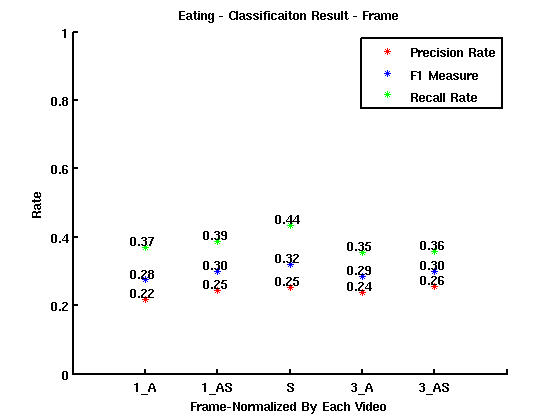
\includegraphics[width=\linewidth]{imgs/Result_Eating_Frame.png}
  \caption{Class Eating - Classification Result of Frame - Frame nomalised by each video}
  \label{fig:REF}
\end{minipage}%
\begin{minipage}{.5\textwidth}
  \centering
  \captionsetup{justification=centering,margin=1cm}
  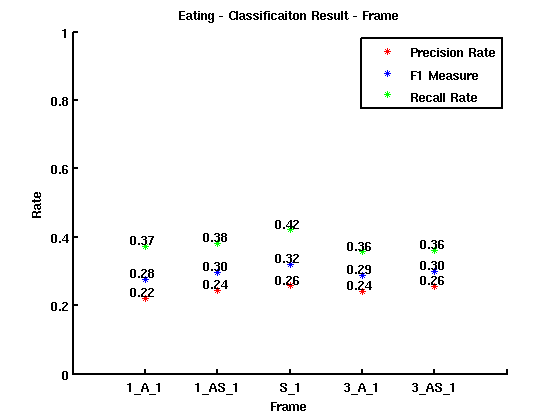
\includegraphics[width=\linewidth]{imgs/Result_Eating_Frame_1.png}
  \caption{Class Eating - Classification Result of Frame - Frame NOT nomalised by each video}
  \label{fig:REF1}
\end{minipage}
\end{figure}
Figure \ref{fig:REF} show precision rate, recall rate and F1 measure of using appearance feature vector that are normalised by each video. Figure \ref{fig:REF} contains result of 5 groups, 1\_A means the appearance feature is extracted by using 1 block uniform pattern and it is using appearance vector for classification. 3\_AS means the appearance feature is extracted by using 3 block uniform pattern and it is using appearance and shape vector for classification. The same for 1\_AS and 3\_A, as using pure shape feature vector, it is not marked as normalised or not normalised. The  largest recall rate and F1 score are obtained by using shape feature vector. There are 
\begin{figure}[ht]
\centering
\begin{minipage}{.5\textwidth}
  \centering
  \captionsetup{justification=centering,margin=1cm}
  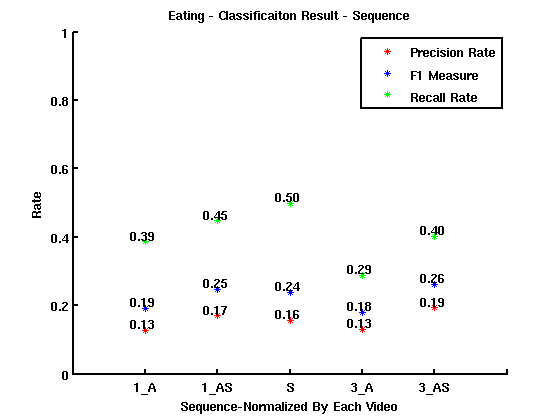
\includegraphics[width=\linewidth]{imgs/Result_Eating_Sequence.png}
  \caption{Class Eating - Classification Result of Frame - Frame nomalised by each video}
  \label{fig:RES}
\end{minipage}%
\begin{minipage}{.5\textwidth}
  \centering
  \captionsetup{justification=centering,margin=1cm}
  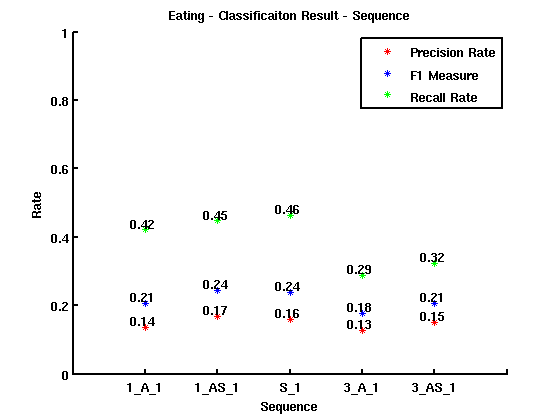
\includegraphics[width=\linewidth]{imgs/Result_Eating_Sequence_1.png}
  \caption{Class Eating - Classification Result of Frame - Frame NOT nomalised by each video}
  \label{fig:RES1}
\end{minipage}
\end{figure}

\begin{figure}[ht]
\centering
\begin{minipage}{.5\textwidth}
  \centering
  \captionsetup{justification=centering,margin=1cm}
  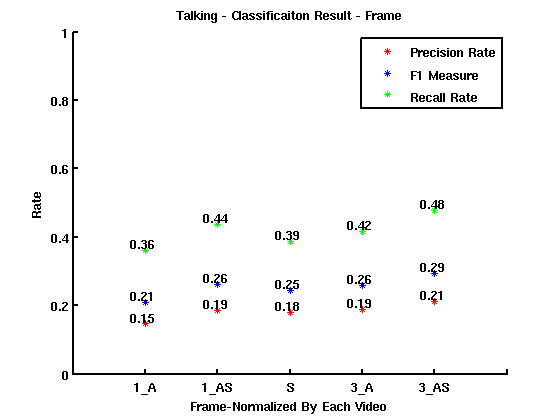
\includegraphics[width=\linewidth]{imgs/Result_Talking_Frame.png}
  \caption{Class Talking - Classification Result of Frame - Frame nomalised by each video}
  \label{fig:RTF}
\end{minipage}%
\begin{minipage}{.5\textwidth}
  \centering
  \captionsetup{justification=centering,margin=1cm}
  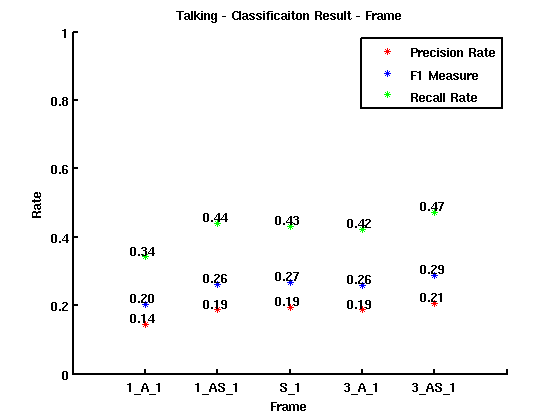
\includegraphics[width=\linewidth]{imgs/Result_Talking_Frame_1.png}
  \caption{Class Talking - Classification Result of Frame - Frame NOT nomalised by each video}
  \label{fig:RTF1}
\end{minipage}
\end{figure}

\begin{figure}[ht]
\centering
\begin{minipage}{.5\textwidth}
  \centering
  \captionsetup{justification=centering,margin=1cm}
  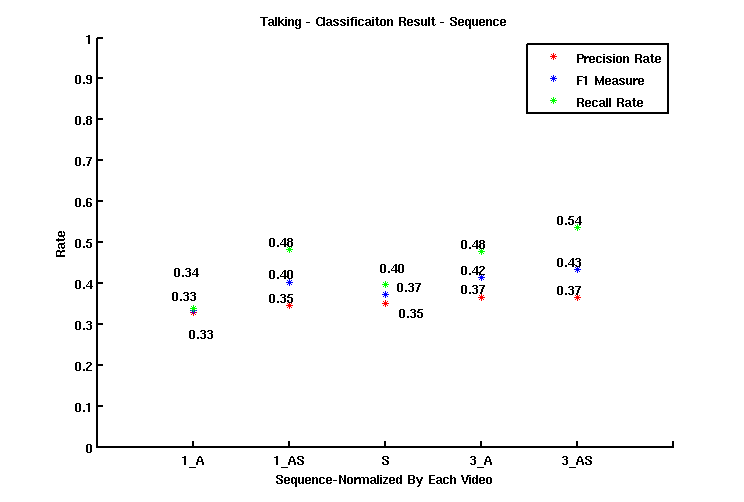
\includegraphics[width=\linewidth]{imgs/Result_Talking_Sequence.png}
  \caption{Class Talking - Classification Result of Sequence - Frame nomalised by each video}
  \label{fig:RTS}
\end{minipage}%
\begin{minipage}{.5\textwidth}
  \centering
  \captionsetup{justification=centering,margin=1cm}
  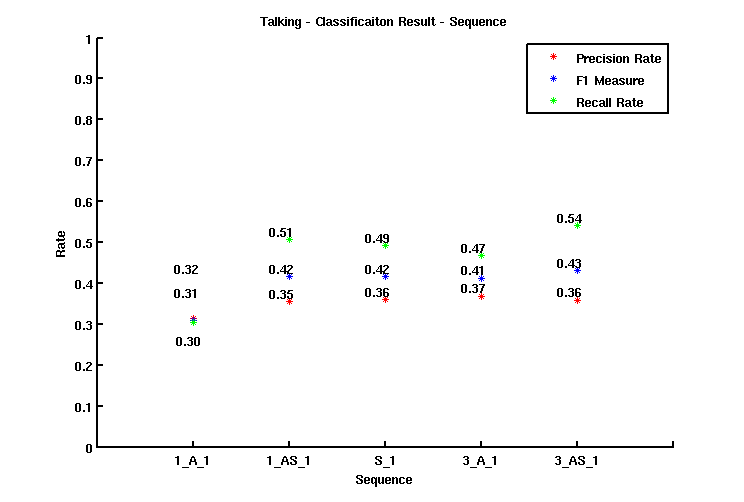
\includegraphics[width=\linewidth]{imgs/Result_Talking_Sequence_1.png}
  \caption{Class Talking - Classification Result of Sequence - Frame NOT nomalised by each video}
  \label{fig:RTS1}
\end{minipage}
\end{figure}

\begin{figure}[ht]
\centering
\begin{minipage}{.5\textwidth}
  \centering
  \captionsetup{justification=centering,margin=1cm}
  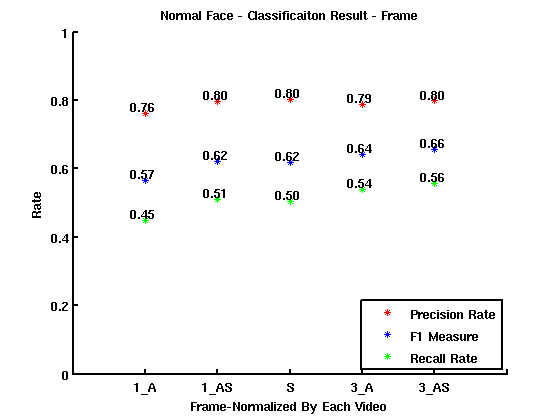
\includegraphics[width=\linewidth]{imgs/Result_NormalFace_Frame.png}
  \caption{Class Normal Face - Classification Result of Frame - Frame nomalised by each video}
  \label{fig:RNF}
\end{minipage}%
\begin{minipage}{.5\textwidth}
  \centering
  \captionsetup{justification=centering,margin=1cm}
  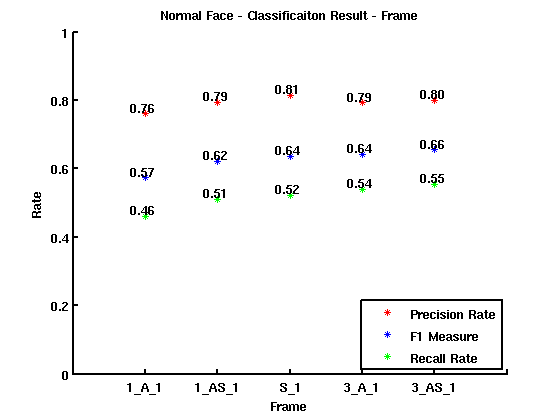
\includegraphics[width=\linewidth]{imgs/Result_NormalFace_Frame_1.png}
  \caption{Class Normal Face - Classification Result of Frame - Frame NOT nomalised by each video}
  \label{fig:RNF1}
\end{minipage}
\end{figure}

\begin{figure}[ht]
\centering
\begin{minipage}{.5\textwidth}
  \centering
  \captionsetup{justification=centering,margin=1cm}
  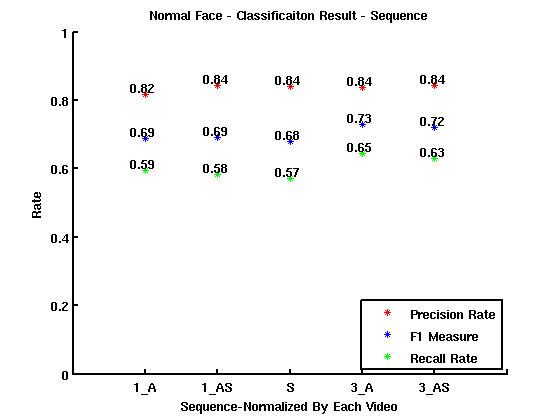
\includegraphics[width=\linewidth]{imgs/Result_NormalFace_Sequence.png}
  \caption{Class Normal Face - Classification Result of Sequence - Frame nomalised by each video}
  \label{fig:RNS}
\end{minipage}%
\begin{minipage}{.5\textwidth}
  \centering
  \captionsetup{justification=centering,margin=1cm}
  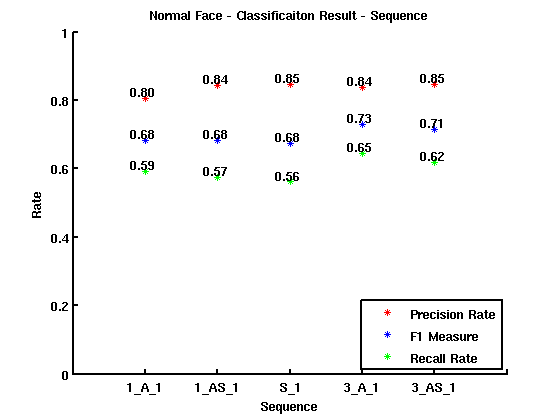
\includegraphics[width=\linewidth]{imgs/Result_NormalFace_Sequence_1.png}
  \caption{Class Normal Face - Classification Result of Sequence - Frame NOT nomalised by each video}
  \label{fig:RNS1}
\end{minipage}
\end{figure}

\begin{figure}[ht]
\centering
\begin{minipage}{.5\textwidth}
  \centering
  \captionsetup{justification=centering,margin=1cm}
  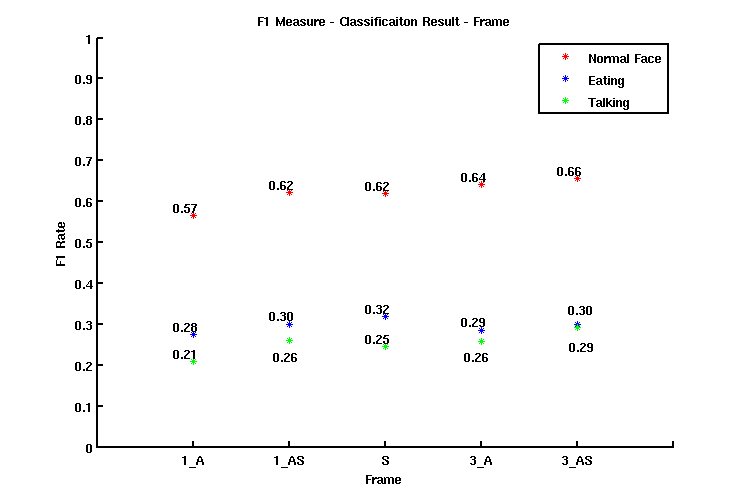
\includegraphics[width=\linewidth]{imgs/Result_F1_Frame.png}
  \caption{Three Class - Classification Result of frame - Frame nomalised by each video}
  \label{fig:RFF}
\end{minipage}%
\begin{minipage}{.5\textwidth}
  \centering
  \captionsetup{justification=centering,margin=1cm}
  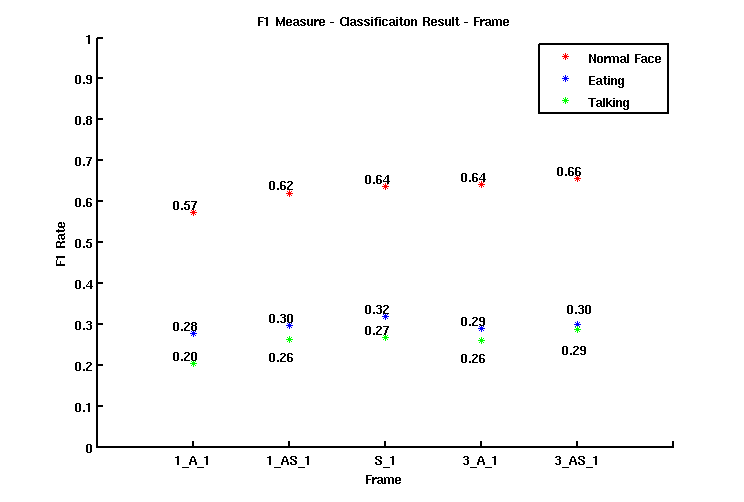
\includegraphics[width=\linewidth]{imgs/Result_F1_Frame_1.png}
  \caption{Three Class - Classification Result of frame - Frame NOT nomalised by each video}
  \label{fig:RFF1}
\end{minipage}
\end{figure}

\begin{figure}[ht]
\centering
\begin{minipage}{.5\textwidth}
  \centering
  \captionsetup{justification=centering,margin=1cm}
  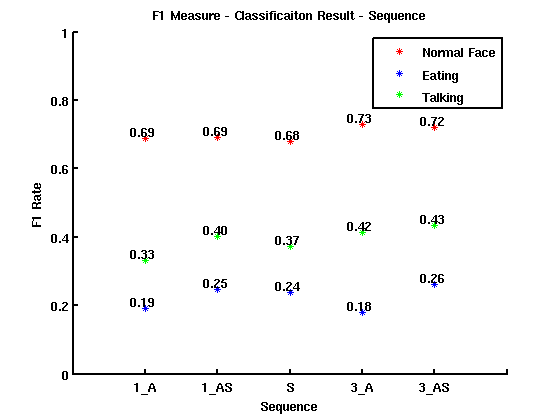
\includegraphics[width=\linewidth]{imgs/Result_F1_Sequence.png}
  \caption{Three Class - Classification Result of frame - Frame nomalised by each video}
  \label{fig:RFS}
\end{minipage}%
\begin{minipage}{.5\textwidth}
  \centering
  \captionsetup{justification=centering,margin=1cm}
  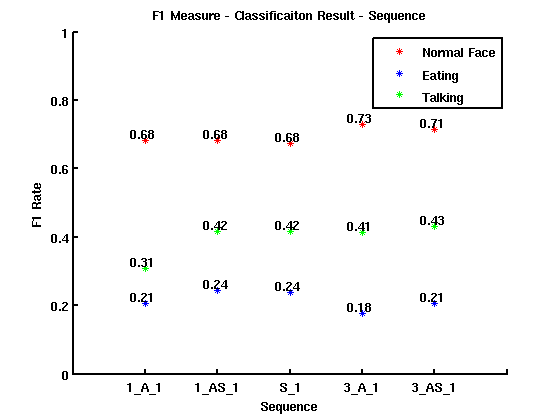
\includegraphics[width=\linewidth]{imgs/Result_F1_Sequence_1.png}
  \caption{Three Class - Classification Result of frame - Frame NOT nomalised by each video}
  \label{fig:RFS1}
\end{minipage}
\end{figure}